\documentclass[aspectratio=169]{beamer}

\usetheme{Boadilla}
\usefonttheme{professionalfonts}
\setbeamertemplate{navigation symbols}{}
\setbeamertemplate{itemize items}[circle]
\setbeamertemplate{enumerate items}[default]
\setbeamertemplate{headline}{}

\usepackage[utf8]{inputenc}
\usepackage[T1]{fontenc}
\usepackage{lmodern}
\usepackage{amsmath}
\usepackage{booktabs}
\usepackage{tabularx}
\usepackage{array}
\usepackage{hyperref}
\usepackage[strings]{underscore}
\usepackage{listings}
\usepackage{tikz}
\usetikzlibrary{arrows.meta,positioning,fit,calc,shapes.geometric}
\usepackage{xcolor}

\definecolor{courseblue}{HTML}{12355B}
\definecolor{coursegold}{HTML}{C98A2E}
\definecolor{courseice}{HTML}{EEF3F8}
\definecolor{coursegreen}{HTML}{2F6B4F}
\definecolor{coursegray}{HTML}{4B5563}
\definecolor{codebg}{HTML}{F7F9FC}
\definecolor{codecomment}{HTML}{5E6C84}
\definecolor{codestring}{HTML}{0B6E4F}

\setbeamercolor{palette primary}{bg=courseblue,fg=white}
\setbeamercolor{palette secondary}{bg=coursegold,fg=white}
\setbeamercolor{palette tertiary}{bg=courseblue,fg=white}
\setbeamercolor{palette quaternary}{bg=coursegold,fg=white}
\setbeamercolor{structure}{fg=courseblue}
\setbeamercolor{frametitle}{bg=courseice,fg=courseblue}
\setbeamercolor{title}{fg=courseblue}
\setbeamercolor{block title}{bg=courseblue,fg=white}
\setbeamercolor{block body}{bg=courseice,fg=black}
\setbeamercolor{normal text}{fg=black,bg=white}
\setbeamercolor{alerted text}{fg=coursegold}

\setbeamerfont{footline}{size=\scriptsize}

\setbeamertemplate{footline}{
  \leavevmode
  \hbox{
    \begin{beamercolorbox}[wd=.33\paperwidth,ht=2.8ex,dp=1.2ex,leftskip=0.8em]{palette primary}%
      University of Trieste
    \end{beamercolorbox}%
    \begin{beamercolorbox}[wd=.49\paperwidth,ht=2.8ex,dp=1.2ex,center]{palette tertiary}%
      \coursename{} \textbar{} \coursecode
    \end{beamercolorbox}%
    \begin{beamercolorbox}[wd=.18\paperwidth,ht=2.8ex,dp=1.2ex,rightskip=0.8em plus1fil]{palette secondary}%
      \insertframenumber{} / \inserttotalframenumber
    \end{beamercolorbox}%
  }
}

\hypersetup{
  colorlinks=true,
  linkcolor=courseblue,
  urlcolor=coursegreen
}

\lstdefinestyle{coursepython}{
  language=Python,
  basicstyle=\ttfamily\footnotesize,
  keywordstyle=\color{courseblue}\bfseries,
  commentstyle=\color{codecomment}\itshape,
  stringstyle=\color{codestring},
  showstringspaces=false,
  columns=fullflexible,
  keepspaces=true,
  frame=single,
  framerule=0.6pt,
  rulecolor=\color{courseblue},
  backgroundcolor=\color{codebg},
  xleftmargin=0.4em,
  xrightmargin=0.4em,
  aboveskip=0.4em,
  belowskip=0.2em
}

\newcommand{\coursename}{Data-driven Systems Engineering}
\newcommand{\coursecode}{440MI / 305SM}
\newcommand{\coursefooter}{}

\newcommand{\learninggoals}[1]{
  \begin{block}{Learning goals}
  #1
  \end{block}
}

\newcommand{\repoactivity}[1]{
  \begin{block}{Repo activity}
  #1
  \end{block}
}

\newcommand{\readinglist}[1]{
  \begin{block}{Papers and materials}
  {\footnotesize #1}
  \end{block}
}

\newcommand{\coursecontextframe}[5]{
  \begin{frame}{Course Map and Running Cases}
  \centering
  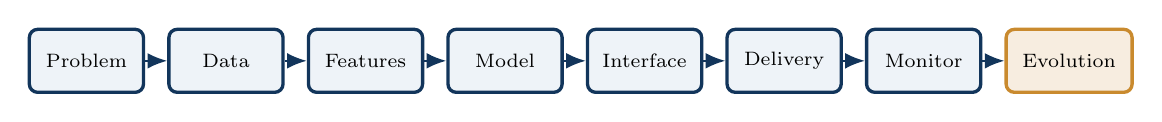
\begin{tikzpicture}[node distance=0.28cm]
  \node[flowbox, minimum width=1.45cm, minimum height=0.8cm] (problem) {\scriptsize Problem};
  \node[flowbox, minimum width=1.45cm, minimum height=0.8cm, right=of problem] (data) {\scriptsize Data};
  \node[flowbox, minimum width=1.45cm, minimum height=0.8cm, right=of data] (features) {\scriptsize Features};
  \node[flowbox, minimum width=1.45cm, minimum height=0.8cm, right=of features] (model) {\scriptsize Model};
  \node[flowbox, minimum width=1.45cm, minimum height=0.8cm, right=of model] (interface) {\scriptsize Interface};
  \node[flowbox, minimum width=1.45cm, minimum height=0.8cm, right=of interface] (delivery) {\scriptsize Delivery};
  \node[flowbox, minimum width=1.45cm, minimum height=0.8cm, right=of delivery] (monitor) {\scriptsize Monitor};
  \node[accentbox, minimum width=1.6cm, minimum height=0.8cm, right=of monitor] (evolution) {\scriptsize Evolution};
  \foreach \a/\b in {problem/data,data/features,features/model,model/interface,interface/delivery,delivery/monitor,monitor/evolution} {
    \draw[arrow] (\a) -- (\b);
  }
  \end{tikzpicture}

  \vspace{0.5em}
  \begin{block}{Today in the course}
  \textbf{Focus:} #1

  \textbf{Bridge:} #2
  \end{block}

  \begin{columns}[T]
  \column{0.48\textwidth}
  \begin{block}{Fraud case}
  {\footnotesize #3}
  \end{block}
  \column{0.48\textwidth}
  \begin{block}{Pasteurization case}
  {\footnotesize #4}
  \end{block}
  \end{columns}

  \vspace{0.3em}
  {\footnotesize \textbf{Course thread:} #5}
  \coursefooter
  \end{frame}
}

\newcommand{\classclosingframe}[4]{
  \begin{frame}{From This Class to the Next}
  \begin{block}{What stays with us}
  #1
  \end{block}

  \begin{columns}[T]
  \column{0.48\textwidth}
  \begin{block}{Project use}
  {\footnotesize #2}
  \end{block}
  \column{0.48\textwidth}
  \begin{block}{Next connection}
  {\footnotesize #3}
  \end{block}
  \end{columns}

  \vspace{0.3em}
  {\footnotesize \textbf{Course thread:} #4}
  \coursefooter
  \end{frame}
}

\tikzset{
  flowbox/.style={
    rounded corners=3pt,
    draw=courseblue,
    fill=courseice,
    very thick,
    minimum width=2.2cm,
    minimum height=0.9cm,
    align=center,
    font=\small
  },
  accentbox/.style={
    rounded corners=3pt,
    draw=coursegold,
    fill=coursegold!15,
    very thick,
    minimum width=2.2cm,
    minimum height=0.9cm,
    align=center,
    font=\small
  },
  arrow/.style={
    -{Latex[length=2.5mm,width=2mm]},
    thick,
    draw=courseblue
  }
}


\title{Class 12: Agile Toolkit for Data and ML Teams}
\author{\coursename}
\date{}

\begin{document}

\frame{\titlepage \coursefooter}

\begin{frame}{Agenda}
\begin{itemize}
\item Collaboration and communication
\item Development practices
\item Planning and tracking
\item Agile frameworks and roles
\item Feedback and customer involvement
\item Agile anti-patterns in data and ML teams
\end{itemize}
\coursefooter
\end{frame}

\begin{frame}{Agile practices are only useful if they change behavior}
\learninggoals{
\begin{itemize}
\item Use ceremonies and artifacts as coordination tools, not rituals.
\item Adapt user stories, estimation, and boards to data-intensive projects.
\item Connect agile practices to quality, deployment, and stakeholder learning.
\item Recognize where standard agile templates break down in exploratory ML work.
\end{itemize}
}
\coursefooter
\end{frame}

\coursecontextframe
{Day-to-day agile coordination for data and ML work.}
{This class turns process-model ideas into concrete planning, review, and feedback practices that teams can actually use.}
{In the fraud case, agile work means slicing the backlog across data checks, model tuning, API behavior, and validation evidence.}
{In the pasteurization case, agile work means making sensor issues, drift tasks, dashboard improvements, and monitoring criteria visible on the board.}
{The thread is that agile only helps when it improves coordination across the full ML lifecycle rather than only speeding up coding.}

\begin{frame}{Agile toolkit means a set of coordination mechanisms}
\begin{itemize}
\item Meetings, boards, stories, and metrics are not the goal of agility.
\item Their value comes from making priorities visible, reducing blockers, and shortening feedback loops.
\item In ML teams, they also help coordinate data work, experimentation, software integration, and operations.
\end{itemize}
\coursefooter
\end{frame}

\begin{frame}{Which agile tools fit ML projects best?}
\begin{itemize}
\item Sprint planning for defining a thin vertical slice.
\item Backlog refinement for clarifying data dependencies and acceptance criteria.
\item Daily stand-ups for surfacing blockers such as missing labels or broken environments.
\item Retrospectives for process improvement, especially around experimentation waste.
\end{itemize}
\coursefooter
\end{frame}

\begin{frame}{Collaboration rituals and what they actually solve}
\begin{tabularx}{\textwidth}{>{\bfseries}l X}
Practice & Practical value \\
\toprule
Sprint planning & Aligns ambition with capacity and dependencies. \\
Daily stand-up & Surfaces blockers before they become schedule failures. \\
Backlog refinement & Prevents ambiguous work from entering a sprint. \\
Retrospective & Improves the way the team works, not only what it built. \\
Review or demo & Tests whether the increment creates stakeholder value. \\
\bottomrule
\end{tabularx}
\coursefooter
\end{frame}

\begin{frame}{Development practices that matter most}
\begin{itemize}
\item Test-driven development for stable service behavior.
\item CI for repeated checks on code and packaging.
\item CD for safe release preparation.
\item Pair review for notebooks, requirements, and production code.
\item Retrospectives for process correction, not blame.
\end{itemize}
\coursefooter
\end{frame}

\begin{frame}{Development practices for notebook-heavy teams}
\begin{itemize}
\item Review notebooks for reproducibility, not only for narrative clarity.
\item Move repeated feature logic into modules before it spreads across files.
\item Treat data validation and schema checks as quality work, not optional cleanup.
\item Use small pull requests so code review remains meaningful.
\end{itemize}
\begin{block}{Course link}
This is where agile meets the software engineering and MLOps parts of the course: speed without quality creates faster confusion.
\end{block}
\coursefooter
\end{frame}

\begin{frame}{Better user stories for this course}
\begin{block}{Weak}
As a student, I want an AI model.
\end{block}
\begin{block}{Better}
As a quality engineer, I want to detect abnormal temperature trajectories during HeatUp so that I can inspect the pasteurization line before product quality drops.
\end{block}
\coursefooter
\end{frame}

\begin{frame}{A better user story also needs acceptance criteria}
\begin{block}{Story}
As a quality engineer, I want abnormal HeatUp trajectories flagged so that I can inspect the pasteurization line before product quality drops.
\end{block}
\begin{block}{Acceptance criteria}
\begin{itemize}
\item The system ingests live or simulated sensor points.
\item It displays the current state and a risk flag.
\item Alerts are logged with timestamp and model version.
\item A false-positive threshold is agreed with stakeholders.
\end{itemize}
\end{block}
\coursefooter
\end{frame}

\begin{frame}{Planning and tracking tools}
\begin{itemize}
\item Kanban boards for work visibility and WIP control.
\item User stories with acceptance criteria.
\item Story points for relative complexity, not exact duration.
\item Burndown and velocity as team learning tools, not performance theater.
\end{itemize}
\coursefooter
\end{frame}

\begin{frame}{A Kanban board adapted to ML work}
\centering
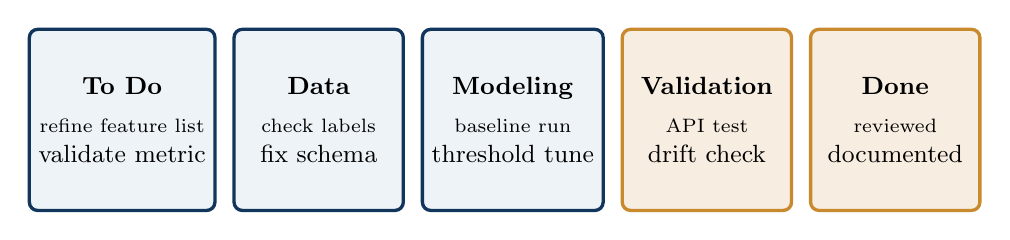
\begin{tikzpicture}[node distance=0.2cm]
\node[flowbox, minimum width=2.15cm, minimum height=2.3cm] (todo) {\textbf{To Do}\\[0.3em]\scriptsize refine feature list\\validate metric};
\node[flowbox, minimum width=2.15cm, minimum height=2.3cm, right=of todo] (data) {\textbf{Data}\\[0.3em]\scriptsize check labels\\fix schema};
\node[flowbox, minimum width=2.15cm, minimum height=2.3cm, right=of data] (model) {\textbf{Modeling}\\[0.3em]\scriptsize baseline run\\threshold tune};
\node[accentbox, minimum width=2.15cm, minimum height=2.3cm, right=of model] (valid) {\textbf{Validation}\\[0.3em]\scriptsize API test\\drift check};
\node[accentbox, minimum width=2.15cm, minimum height=2.3cm, right=of valid] (done) {\textbf{Done}\\[0.3em]\scriptsize reviewed\\documented};
\end{tikzpicture}
\vspace{0.5em}
\begin{itemize}
\item This kind of board makes hidden data work visible instead of pretending every task is pure coding.
\end{itemize}
\coursefooter
\end{frame}

\begin{frame}{Planning tools students can actually use}
\begin{itemize}
\item Kanban board with columns for data, modeling, integration, and validation.
\item Story points only after the team shares a definition of complexity.
\item Burndown charts for sprint scope, not for pretending uncertainty does not exist.
\item Definition of Ready and Definition of Done for every deliverable.
\end{itemize}
\coursefooter
\end{frame}

\begin{frame}{Estimation is for coordination, not prediction theater}
\begin{itemize}
\item Story points work best as a relative complexity language shared by the team.
\item Estimation fails when people use points as disguised hours.
\item High uncertainty tasks should often be split into investigation work before full implementation.
\item Velocity should guide planning, not evaluate people.
\end{itemize}
\coursefooter
\end{frame}

\begin{frame}{Agile meets DevOps and MLOps}
\begin{itemize}
\item Continuous integration protects the code path.
\item Continuous delivery protects the release path.
\item Monitoring closes the loop after release.
\item Without operational feedback, agile becomes local optimization.
\end{itemize}
\coursefooter
\end{frame}

\begin{frame}{Frameworks and their natural use}
\begin{columns}[T]
\column{0.48\textwidth}
\textbf{Structured rhythm}
\begin{itemize}
\item Scrum for bounded sprint goals
\item Good for student teams needing cadence
\item Useful when review moments matter
\end{itemize}
\column{0.48\textwidth}
\textbf{Flow orientation}
\begin{itemize}
\item Kanban for continuous incoming work
\item Good for ops-heavy or support-heavy teams
\item Useful when work types vary a lot
\end{itemize}
\end{columns}
\vspace{0.5em}
\begin{block}{Bridge}
DevOps and MLOps extend both by asking how work is built, shipped, observed, and improved after release.
\end{block}
\coursefooter
\end{frame}

\begin{frame}{Frameworks and roles}
\begin{itemize}
\item Scrum: structured events, roles, and sprint rhythm.
\item Kanban: flow-oriented work management.
\item DevOps: shared responsibility across build, release, and operations.
\item MLOps: extends DevOps with data, models, drift, and governance concerns.
\end{itemize}
\coursefooter
\end{frame}

\begin{frame}{Agile anti-patterns in data teams}
\begin{itemize}
\item Treating research uncertainty as if it were ordinary feature implementation.
\item Filling sprints with vaguely defined ``improve model'' tasks.
\item Ignoring data dependencies until late integration.
\item Using demos that show only happy-path notebooks instead of operational evidence.
\item Running retrospectives that identify problems but never change behavior.
\end{itemize}
\coursefooter
\end{frame}

\begin{frame}{What good agile behavior looks like in this course}
\repoactivity{
\begin{itemize}
\item Use notebooks to explore, then promote reusable logic into scripts or services.
\item Demonstrate thin slices such as ingest plus baseline plus API rather than isolated fragments.
\item Keep project boards aligned with requirements, deployment work, and monitoring plans.
\item Show how feedback changes backlog priorities instead of pretending the first plan was complete.
\end{itemize}
}
\coursefooter
\end{frame}

\classclosingframe
{\begin{itemize}
\item Agile in data-driven work means learning quickly while preserving evidence and alignment.
\item Stories, boards, demos, and retrospectives are useful only when they reflect technical and data reality.
\item Thin vertical slices are stronger than isolated notebook achievements.
\end{itemize}}
{Teams should now be able to organize milestones, backlog items, and reviews around deployable progress instead of vague promises to improve the model later.}
{Class 13 reconnects these practices to MLOps, where experimentation, delivery, ownership, and monitoring become one operational system.}
{Agile coordination gives the team a way to move continuously; MLOps gives that movement technical reliability.}

\begin{frame}{Papers and materials}
\readinglist{
\href{https://www.scrumguides.org/}{Scrum Guide};\ 
\href{https://kanban.university/kanban-resources/getting-started/what-is-kanban/}{What is Kanban};\ 
\href{https://www.oreilly.com/library/view/learning-agile/9780596527679/}{Learning Agile};\ 
\href{https://martinfowler.com/bliki/UserStory.html}{Martin Fowler on user stories};\ 
\href{https://itrevolution.com/product/accelerate/}{Forsgren, Humble, Kim, Accelerate}.
}
\coursefooter
\end{frame}

\end{document}
